\subsection{Überblick}
DYCOS (\underline{DY}namic \underline{C}lassification 
algorithm with c\underline{O}ntent and \underline{S}tructure) ist ein 
Knotenklassifizierungsalgorithmus, der Ursprünglich in \cite{aggarwal2011} vorgestellt 
wurde. Er klassifiziert Knoten, indem mehrfach Random Walks startend
bei dem zu klassifizierenden Knoten gemacht werden und die Labels
der besuchten Knoten gezählt werden. Das Label, das am häufigsten
vorgekommen ist, wird zur Klassifizierung verwendet.
Der DYCOS-Algorithmus nimmt jedoch nicht einfach den Graphen für 
dieses Verfahren, sondern erweitert ihn mit Hilfe der zur Verfügung
stehenden Texte.

Für diese Erweiterung wird zuerst wird Vokabular $W_t$ bestimmt, das 
charakteristisch für eine Knotengruppe ist. Wie das gemacht werden kann
und warum nicht einfach jedes Wort in das Vokabular aufgenommen wird,
wird in Abschnitt~\ref{sec:vokabularbestimmung} erläutert.\\
Nach der Bestimmung des Vokabulars wird für 
jedes Wort im Vokabular ein Wortknoten zum Graphen hinzugefügt. Alle
Knoten, die der Graph zuvor hatte, werden nun \enquote{Strukturknoten}
genannt.
Ein Strukturknoten $v$ wird genau dann mit einem Wortknoten $w \in W_t$
verbunden, wenn $w$ in einem Text von $v$ vorkommt.

\begin{figure}[htp]
    \centering
    \tikzstyle{vertex}=[draw,black,circle,minimum size=10pt,inner sep=0pt]
\tikzstyle{edge}=[very thick]
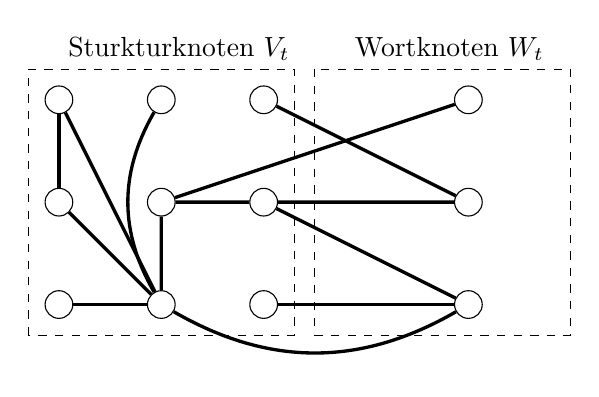
\begin{tikzpicture}[scale=1.3]
    \node (a)[vertex] at (0,0) {};
    \node (b)[vertex]  at (0,1) {};
    \node (c)[vertex] at (0,2) {};
    \node (d)[vertex] at (1,0) {};
    \node (e)[vertex]  at (1,1) {};
    \node (f)[vertex] at (1,2) {};
    \node (g)[vertex] at (2,0) {};
    \node (h)[vertex] at (2,1) {};
    \node (i)[vertex] at (2,2) {};

    \node (x)[vertex] at (4,0) {};
    \node (y)[vertex] at (4,1) {};
    \node (z)[vertex] at (4,2) {};

    \draw[edge] (a) -- (d);
    \draw[edge] (b) -- (d);
    \draw[edge] (b) -- (c);
    \draw[edge] (c) -- (d);
    \draw[edge] (d) -- (e);
    \draw[edge] (d) edge[bend left] (f);
    \draw[edge] (d) edge[bend right] (x);
    \draw[edge] (g) edge (x);
    \draw[edge] (h) edge (x);
    \draw[edge] (h) edge (y);
    \draw[edge] (h) edge (e);
    \draw[edge] (e) edge (z);
    \draw[edge] (i) edge (y);

    \draw [dashed] (-0.3,-0.3) rectangle (2.3,2.3);
    \draw [dashed] (2.5,2.3) rectangle (5, -0.3);

    \node (struktur)[label={[label distance=0cm]0:Sturkturknoten $V_t$}] at (-0.1,2.5) {};
    \node (struktur)[label={[label distance=0cm]0:Wortknoten $W_t$}] at (2.7,2.5) {};
\end{tikzpicture}

    \caption{Erweiterter Graph}
    \label{fig:erweiterter-graph}
\end{figure}

Der DYCOS-Algorithmus betrachtet die Texte, die einem Knoten 
zugeornet sind, als eine
Multimenge von Wörtern. Das heißt, zum einen wird nicht auf die
Reihenfolge der Wörter geachtet, zum anderen wird bei Texten
eines Knotens nicht zwischen verschiedenen Texten unterschieden.
Jedoch wird die Anzahl der Vorkommen jedes Wortes berücksichtigt.

\subsection{Datenstrukturen}
Zusätzlich zu dem gerichteten Graphen $G_t = (V_t, E_t, V_{L,t})$ 
verwaltet der DYCOS-Algorithmus zwei weitere Datenstrukturen:
\begin{itemize}
    \item Für jeden Knoten $v \in V_t$ werden die vorkommenden Wörter,
          die auch im Vokabular $W_t$ sind,
          und deren Anzahl gespeichert. Das könnte z.~B. über ein 
          assoziatives Array geschehen. Wörter, die nicht in 
          Texten von $v$ vorkommen, sind nicht im Array. Für
          alle vorkommenden Wörter ist der gespeicherte Wert zum 
          Schlüssel \enquote{Wort} die Anzahl der Vorkommen von 
          \enquote{Wort} in den Texten von $v$.
    \item Für jedes Wort des Vokabulars $W_t$ wird eine Liste von 
          Knoten verwaltet, in deren Texten das Wort vorkommt.
\end{itemize}

\subsection{Algorithmen}
Bevor der Algorithmus formal beschrieben wird, wird eine Definition
des strukturellen $l$-Sprungs benötigt:
\begin{definition}
    Sei $G_{E,t} = (V_t, E_{S,t} \cup E_{W,t}, V_{L,t}, W_{t})$ der
    um die Wortknoten $W_{t}$ erweiterte Graph.

    Dann heißt ein Random Walk der Länge $l$ in diesem Graphen
    ein \textbf{struktureller $l$-Sprung}, wenn für den Random Walk
    nur Kanten aus $E_{S,t}$ benutzt werden.
\end{definition}

Der strukturelle $l$-Sprung ist also ein Random Walk der Länge $l$
im Graph $G_t$. Im Gegensatz dazu benötigt der inhaltliche $l$-Mehrfachsprung
tatsächlich die Grapherweiterung:

\begin{definition}
    Sei $G_t = (V_t, E_{S,t} \cup E_{W,t}, V_{L,t}, W_{t})$ der
    um die Wortknoten $W_{t}$ erweiterte Graph.

    Dann heißt ein Random Walk der Länge $l$ in diesem Graphen
    ein \textbf{inhaltlicher $l$-Mehrfachsprung}, wenn für den Random Walk
    in jedem der $l$ Schritte, startend von einem Knoten $v \in V_t$
    eine Kante zu einem Wortknoten und von dem Wortknoten wieder 
    zu einem Strukturknoten genommen wird.
\end{definition}

\begin{algorithm}[H]
    \begin{algorithmic}
        \Require \\$\G_t = (\N_t, \A_t, \T_t)$ (Netzwerk),\\
                 $r$ (Anzahl der Random Walks),\\
                 $l$ (Länge eines Random Walks),\\
                 $p_s$ (Wahrscheinlichkeit eines strukturellen Sprungs)
        \Ensure  Klassifikation von $\N_t \setminus \T_t$\\

        \Procedure{SturkturellerSprung}{Dictionary $d$, Startknoten $v$, Länge $l$}
            \For{$i$ von $1$ bis $l$}
                \State $v \gets v.\Call{Next}{}$
                \ForAll{Label $w$ in v.\Call{GetLabels}{}}
                    \State $d[w] = d[w] + 1$
                \EndFor
            \EndFor
        \EndProcedure
        \\
        \Procedure{InhaltlicherMehrfachsprung}{Dictionary $d$, Startknoten $v$, Länge $l$}
            \For{$i$ von $1$ bis $l$}
                \State $v \gets v.\Call{Next}{}$ \Comment{TODO: Hier muss ein mehrfachsprung beschrieben werden!}
                \ForAll{Label $w$ in v.\Call{GetLabels}{}}
                    \State $d[w] = d[w] + 1$
                \EndFor
            \EndFor
        \EndProcedure
        \\

        \ForAll{Knoten $v$ in $\N_t \setminus \T_t$}
            \State $d \gets $ Dictionary, das für neue Einträge 0 annimmt
            \For{$i$ von $1$ bis $r$}
                \State $sprungTyp \gets \Call{random}{0, 1}$
                \If{$sprungTyp \leq p_S$}
                    \State \Call{SturkturellerSprung}{$v$, $l$}
                \Else
                    \State \Call{InhaltlicherMehrfachsprung}{$v$, $l$}
                \EndIf
            \EndFor
            \State $label \gets \Call{max}{d}$
            \State $v.\Call{SetLabel}{label}$
        \EndFor
        \State \Return Labels für $\N_t \setminus \T_t$
    \end{algorithmic}
\caption{DYCOS-Algorithmus}
\label{alg:DYCOS}
\end{algorithm}

\subsection{Inhaltliche Mehrfachsprünge}
Es ist nicht sinnvoll, direkt von einem strukturellem Knoten 
$v \in \N_t$ zu einem mit $v$ verbundenen Wortknoten $w$ zu springen
und von diesem wieder zu einem verbundenem strutkurellem Knoten 
$v' \in \N_t$. Würde man dies machen, wäre zu befürchten, dass
aufgrund von Homonymen die Qualität der Klassifizierung verringert
wird. So hat \enquote{Brücke} im Deutschen viele Bedeutungen.
Gemeint sein können z.~B. das Bauwerk, das Entwurfsmuster der
objektorientierten Programmierung oder ein Teil des Gehirns.

Deshalb wird für jeden Knoten $v$, von dem aus man einen inhaltlichen
Mehrfachsprung machen will folgendes vorgehen gewählt:
\begin{enumerate}
    \item Gehe alle in $v$ startenden Random Walks der Länge 2 durch
          und erstelle eine Liste $L$, der erreichbaren Knoten $v'$. Speichere
          außerdem, durch wie viele Pfade diese Knoten $v'$ jeweils erreichbar sind.
    \item Betrachte im folgenden nur die Top-$q$ Knoten, wobei $q \in \mathbb{N}$
          eine zu wählende Konstante des Algorithmus ist.
    \item Wähle mit Wahrscheinlichkeit $\frac{\Call{Anzahl}{v'}}{\sum_{w \in L} \Call{Anzahl}{v'}}$
          den Knoten $v'$ als Ziel des Mehrfachsprungs.
\end{enumerate}

\subsection{Vokabularbestimmung}\label{sec:vokabularbestimmung}
Da die Größe des Vokabulars die Datenmenge signifikant beeinflusst,
liegt es in unserem Interesse so wenig Wörter wie möglich ins
Vokabular aufzunehmen. Insbesondere sind Wörter nicht von Interesse,
die in fast allen Texten vorkommen, wie im Deutschen z.~B.
\enquote{und}, \enquote{mit} und die Pronomen. Es ist wünschenswert
Wörter zu wählen, die die Texte möglichst stark voneinander Unterscheiden.
Der DYCOS-Algorithmus wählt die Top-$m$ dieser Wörter als Vokabular,
wobei $m \in \mathbb{N}$ eine Festzulegende Konstante ist. In \cite[S. 365]{aggarwal2011}
wird der Einfluss von $m \in \Set{5,10, 15,20}$ auf die Klassifikationsgüte
untersucht und festgestellt, dass die Klassifikationsgüte mit größerem
$m$ sinkt, sie also für $m=5$ für den DBLP-Datensatz am höchsten ist.
Für den CORA-Datensatz wurde mit $m \in \set{3,4,5,6}$ getestet und 
kein signifikanter Unterschied festgestellt.

Nun kann man manuell eine Liste von zu beachtenden Wörtern erstellen
oder mit Hilfe des Gini-Koeffizienten automatisch ein Vokabular erstellen.
Der Gini-Koeffizient ist ein statistisches Maß, das die Ungleichverteilung
bewertet. Er ist immer im Intervall $[0,1]$, wobei $0$ einer 
Gleichverteilung entspricht und $1$ der größtmöglichen Ungleichverteilung.

Sei nun $n_i(w)$ die Häufigkeit des Wortes $w$ in allen Texten mit 
der $i$-ten Knotenbeschriftung.
\begin{align}
    p_i(w) &:= \frac{n_i(w)}{\sum_{j=1}^{|\L_t|} n_j(w)} &\text{(Relative Häufigkeit des Wortes $w$)}\\
    G(w)   &:= \sum_{j=1}^{|\L_t|} p_j(w)^2              &\text{(Gini-Koeffizient von $w$)}
\end{align}
In diesem Fall ist $G(w)=0$ nicht möglich, da zur Vokabularbestimmung
nur Wörter betrachtet werden, die auch vorkommen.

Ein Vorschlag, wie die Vokabularbestimmung implementiert werden kann,
ist als Pseudocode mit \cref{alg:vokabularbestimmung}
gegeben. Dieser Algorithmus benötigt neben dem Speicher für den
Graphen, die Texte sowie die $m$ Vokabeln noch $\mathcal{O}(|\text{Verschiedene Wörter in } S_t| \cdot (|\L_t| + 1))$
Speicher. Die Average-Case Zeitkomplexität beträgt 
$\mathcal{O}(|\text{Wörter in } S_t|)$, wobei dazu die Vereinigung
von Mengen $M,N$ in $\mathcal{O}(\min{|M|, |N|})$ sein muss.

\begin{algorithm}
    \begin{algorithmic}[1]
        \Require \\
                 $V_{L,t}$ (beschriftete Knoten),\\
                 $\L_t$ (Beschriftungen),\\
                 $f:V_{L,t} \rightarrow \L_t$ (Beschriftungsfunktion),\\
                 $m$ (Gewünschte Vokabulargröße)
        \Ensure  $\M_t$ (Vokabular)\\

        \State $S_t \gets \Call{Sample}{V_{L,t}}$ \Comment{Wähle eine Teilmenge $S_t \subseteq V_{L,t}$ aus}
        \State $\M_t \gets \bigcup_{v \in S_t} \Call{getTextAsSet}{v}$ \Comment{Menge aller Wörter}
        \State $cLabelWords \gets (|\L_t|+1) \times |\M_t|$-Array, mit 0en initialisiert\\

        \ForAll{$v \in V_{L,t}$} \Comment{Gehe jeden Text Wort für Wort durch}
            \State $i \gets \Call{getLabel}{v}$
            \ForAll{$(word, occurences) \in \Call{getTextAsMultiset}{v}$}
                \State $cLabelWords[i][word] \gets cLabelWords[i][word] + occurences$
                \State $cLabelWords[i][|\L_t|] \gets cLabelWords[i][|\L_t|] + occurences$
            \EndFor
        \EndFor
        \\
        \ForAll{Wort $w \in \M_t$}
            \State $p \gets $ Array aus $|\L_t|$ Zahlen in $[0, 1]$
            \ForAll{Label $i \in \L_t$}
                \State $p[i] \gets \frac{cLabelWords[i][w]}{cLabelWords[i][|\L_t|]}$
            \EndFor

            \State $w$.gini $\gets 0$
            \ForAll{$i \in 1, \dots, |\L_t|$}
                \State $w$.gini $\gets$ $w$.gini + $p[i]^2$
            \EndFor
        \EndFor

        \State $\M_t \gets \Call{SortDescendingByGini}{\M_t}$
        \State \Return $\Call{Top}{\M_t, m}$
    \end{algorithmic}
\caption{Vokabularbestimmung}
\label{alg:vokabularbestimmung}
\end{algorithm}

Die Menge $S_t$ kann aus der Menge aller Dokumente, deren 
Knoten beschriftet sind, mithilfe des in \cite{Vitter} vorgestellten
Algorithmus bestimmt werden.

